\documentclass[tikz,border=10pt]{standalone}
\usepackage{tikz}
\usetikzlibrary{calc}

\begin{document}
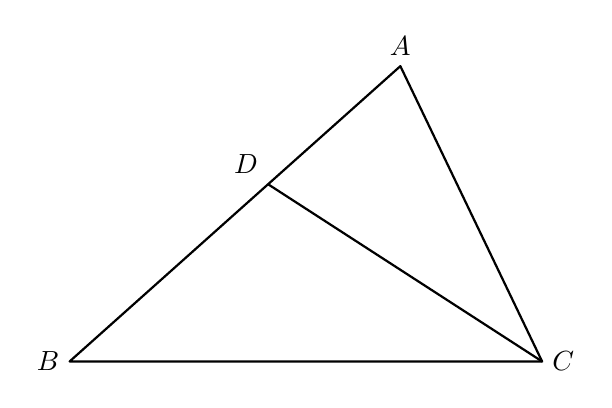
\begin{tikzpicture}[thick, line join=round, line cap=round, scale=1.5]
    % 1. 定义顶点坐标 (基于图像比例估算)
    \coordinate (B) at (0,0);
    \coordinate (C) at (4,0);
    \coordinate (A) at (2.8,2.5);
    
    % 2. 定义边上的点 D (位于 AB 边上，约 0.6 比例处)
    \coordinate (D) at ($(A)!0.4!(B)$); 

    % 3. 绘制三角形主体
    \draw (A) -- (B) -- (C) -- cycle;

    % 4. 绘制内部连线 CD
    \draw (C) -- (D);

    % 5. 标注顶点标签 (使用 anchor 确保标签不遮挡线条)
    \node [above] at (A) {$A$};
    \node [left]  at (B) {$B$};
    \node [right] at (C) {$C$};
    \node [above left] at (D) {$D$};

\end{tikzpicture}
\end{document}